\section{Cryptoeconomics}

We now present our economic analysis on our client. We have
already discussed that the NIPoPoW protocol is performed in distinct phases. In
each phase, different entities are prompted to act. As in SPV, the security
assumption that is made is that at least one honest node is connected to the
verifier contract and serves honest proofs. However, the process of contesting
a submitted proof by an honest node does not come without expense.  Such an
expense is the computational power a node has to consume in order to fetch a
submitted proof from the calldata and construct a contesting proof, but, most
importantly, the gas that has to be paid in order to dispatch the proof to
the Ethereum blockchain. Therefore, it is essential to provide incentives to
honest nodes, while adversaries must be discouraged from
submitting invalid proofs. In this section, we discuss the topic of incentives
and treat our honest nodes as rational. We propose concrete monetary values
to achieve incentive compatibility.

In NIPoPoWs, incentive compatibility is addressed by the establishment of a monetary value
termed \emph{collateral}. In the \emph{submit} phase, the user pays this collateral in
addition to the expenses of the function call, and, if the proof is contested
successfully, the collateral is paid to the user that successfully invalidated
the proof. If the proof is not contested, then the collateral is returned to
the original issuer. This treatment incentivizes nodes to participate to the
protocol, and discourages adversaries from joining. It is critical that the
collateral covers all the expenses of the entity issuing the contest and in
particular the gas costs of the contestation.

\noindent \textbf{Collateral versus contestation period.}
The contestation period and the collateral are generally inversely proportional quantities
and are both hard-coded in a particular deployment of the NIPoPoW verifier smart contract.
If the contestation period is large, the collateral can be allowed to become small, as
it suffices for any contester to pay a small gas price to ensure the contestation transaction is
confirmed within the contestation period. On the other hand, if the contestation period is
small, the collateral must be made large so as to ensure that it can cover the,
potentially large, gas costs required for quick confirmation. This introduces an expected trade-off
between good liveness (fast availability of cross-chain data ready for consumption) and
cheap collateral (the amount of money that needs to be locked up while the claim is pending).
The balance between the two is a matter of application and is determined by user policy.
Any user of the NIPoPoW
verifier smart contract must at a minimum ensure that the collateral and contestation
period parameters are both lower-bounded in such a way that the smart contract is incentive compatible.
If these bounds are not attained, the aspiring user of the NIPoPoW verifier smart
contract must refuse to use it, as the contract does not provide incentive compatibility
and is therefore not secure. Depending on the application, the user may wish to impose
additional upper bounds on the contestation period (to ensure good liveness) or on the
collateral (to ensure low cost), but these are matters of performance and not security.

\noindent \textbf{Analysis.} We give concrete bounds for the contestation period and
collateral parameters. It is known~\cite{wood} that gas prices affect the prioritization
of transactions within blocks. In particular, each block mined by a rational miner
will contain roughly all transactions of the mempool sorted by decreasing gas price
until a certain minimum gas price is reached. We used the Etherchain
explorer~\cite{etherchain} to download recent blocks and inspected their included
transactions to determine their lowest gas price. In our measurements, we make the
simplifying assumption that miners are rational and therefore will necessarily include
a transaction of higher gas price if they are including a transaction of lower gas price.
We sampled $200$ blocks of the Ethereum blockchain around March 2020 (up to block height $9{,}990{,}025$) and
collected their respective minimum
gas prices.
Starting with a range of reasonable gas prices, and based on our miner rationality assumption,
we modelled the experiment of acceptance of a transaction
with a given gas price within the next block as a Bernoulli trial.
The probability of this distribution is given by the percentage
of block samples among the $200$ which have a lower minimum gas price,
a simple maximum likelihood estimation of the Bernoulli parameter.
This sampling of real data gives the discretized appearance in our graph.
For each of these Bernoulli distributions, and the respective gas price, we deduced
a Geometric distribution modelling the number of blocks that the party must wait
for before their transaction becomes confirmed.

Given these various candidate gas prices (in gwei), and multiplying them by the gas cost
needed to call the NIPoPoW \emph{contest} method, we arrived at an absolute minimum collateral
for each nominal gas price
which is just sufficient to cover the gas cost of the contestation transaction
(real collateral must include some additional compensation to ensure a rational miner
is also compensated for the cost of monitoring the blockchain). For each
of these collaterals, we used the previous geometric distribution to determine both the
\emph{expected} number of blocks needed to wait prior to confirmation, as well as an
upper bound on the number of blocks needed for confirmation. For the purpose of an upper bound, we
plot one standard deviation above the mean. This upper bound corresponds to the minimum
contestation period recommended, as this bound ensures that, at the given gas price,
if the number of blocks needed to wait for falls within one standard deviation of
the geometric distribution mean, then the rational contester will create a transaction that
will become confirmed prior to the contestation period expiring. Critical applications
that require a higher assurance of success must consider larger deviations from the
mean.

We display the cost of submitting a proof in
Figure~\ref{fig:cryptoeconomics-submit}. The horizontal axis shows the cost of
submit in USD and Ether (using ether prices of $1$ ether = $217.41$
USD as of June 2020). The vertical axis shows the number of blocks needed for
at least one confirmation. We observe that $0.50$ USD are
enough to ensure that the submission is confirmed within 5 blocks.

We plot our cryptoeconomic recommendations based on our measurements in
Figure~\ref{fig:cryptoeconomics-collateral}. The horizontal axis shows the collateral denominated in
both Ether and USD (using ether prices of $1$ ether = $246.41$ USD as of June 2020).
We assume that the rational contester will pay a contestation gas cost up to the
collateral itself. The vertical axis shows the recommended contestation period.
The solid line is computed from the block wait time needed for confirmation
according to the mean of the geometric distribution at the given gas price.
The shaded area depicts one standard deviation below and above the mean of
the geometric distribution.

Our experiments are based on the contestation transaction gas cost of the previous
section; namely they are conduced on a blockchain of $650{,}000$ blocks with a NIPoPoW
proof of $250$ blocks. The contesting proof stands at a fork point after which the
original proof deviates with $100$ blocks, while the contesting proof deviates with
$200$ disjoint blocks.

The analysis of this
experiment is displayed in Figure~\ref{fig:cryptoeconomics-collateral-100}. We
also illustrate the expected price of contesting proofs when the fork point of
the adversarial chain is at $Genesis$. Although we claim that this is an
improbable case, we show that the verifier can handle such extreme scenarios.
The analysis of genesis-fork is displayed in
Figure~\ref{fig:cryptoeconomics-collateral-genesis}.

\begin{figure}
    \centering
    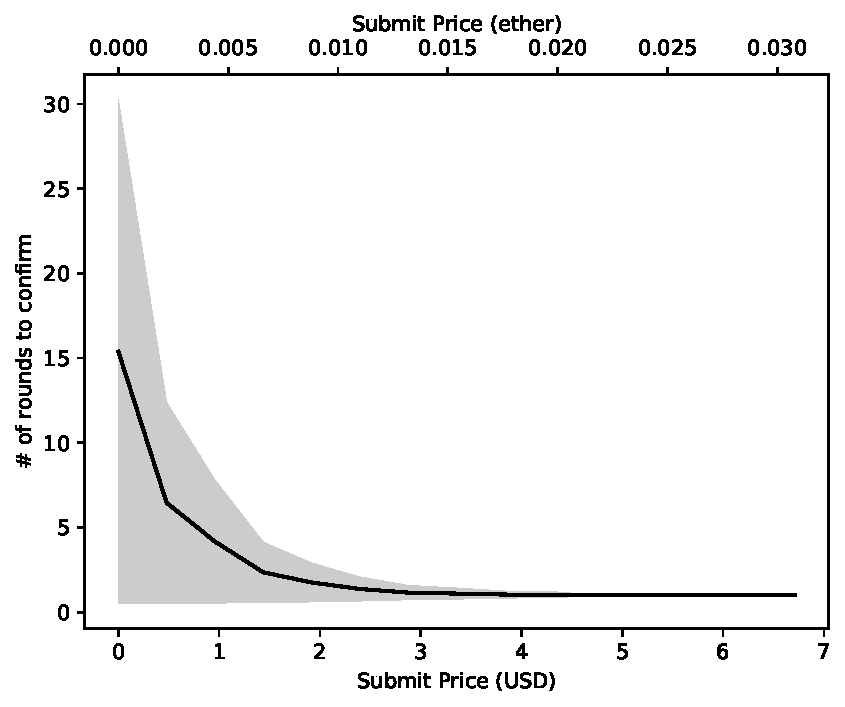
\includegraphics[width=0.7\columnwidth]{figures/cryptoeconomics-submit.pdf}
    \caption{Cost of submitting a NIPoPoW proof.}
    \label{fig:cryptoeconomics-submit}
\end{figure}

\begin{figure}
    \centering
    \begin{subfigure}{0.7\columnwidth}
        \centering
        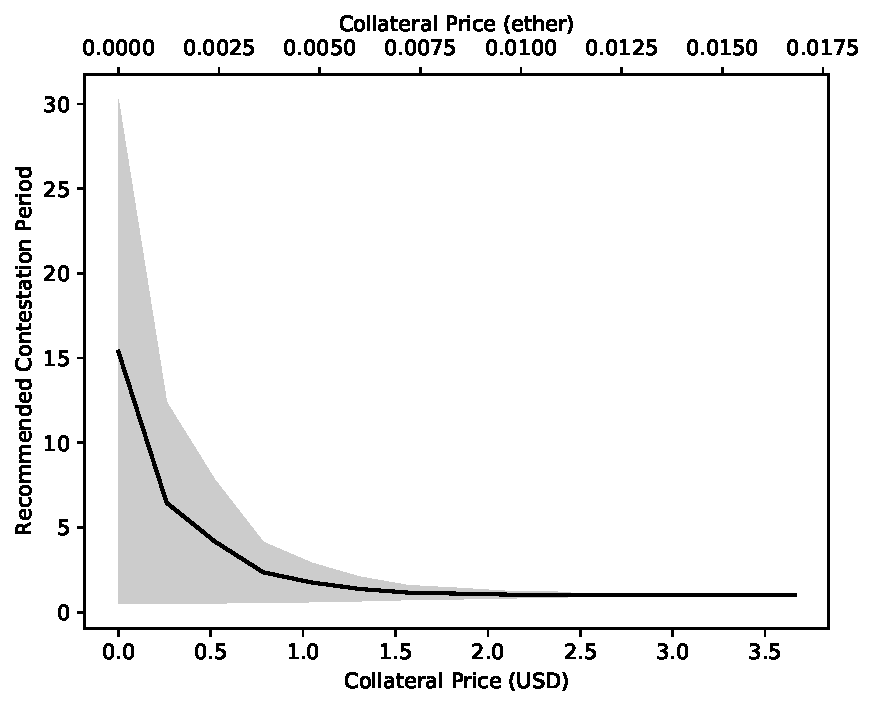
\includegraphics[width=1\columnwidth]{figures/cryptoeconomics-collateral-100.pdf}
        \caption{Cost of collateral when the fork point is 100 blocks prior to the
        tip (expected scenario).}
        \label{fig:cryptoeconomics-collateral-100}
    \end{subfigure}
    \begin{subfigure}{0.7\columnwidth}
        \centering
        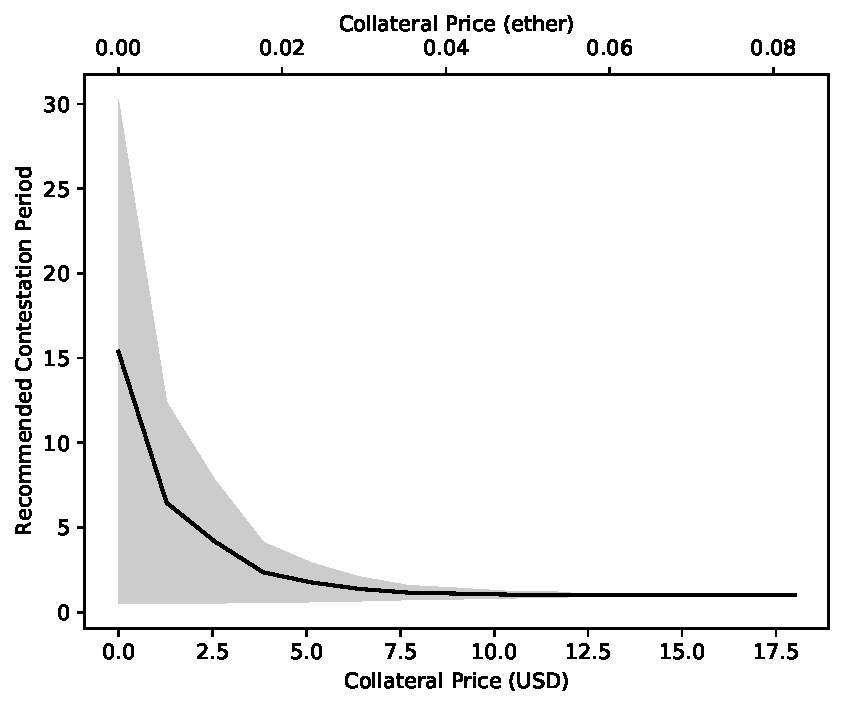
\includegraphics[width=1\columnwidth]{figures/cryptoeconomics-collateral-genesis.pdf}
        \caption{Cost of collateral when the fork point is Genesis (most expensive scenario).}
        \label{fig:cryptoeconomics-collateral-genesis}
    \end{subfigure}
    \caption{Cryptoeconomic recommendations for the NIPoPoW superlight client.}
    \label{fig:cryptoeconomics-collateral}
\end{figure}

We conclude that consumption of cross-chain data within the Ethereum blockchain
can be obtained at very reasonable cost. If the waiting time is set to just
$10$ Ethereum blocks (approximately $2$ minute in expectation), a collateral of
just $0.50$ USD is sufficient to cover for up to one standard deviation in
confirmation time. Note that the collateral of an honest party is not consumed
and is returned to the party upon the expiration of the contestation period. We
therefore deem our implementation to be practical.

